\documentclass[french]{beamer}
\usepackage[round]{natbib}

\usepackage{pgfpages}
%\setbeameroption{show notes}
%\setbeameroption{show notes on second screen=right}
\mode<presentation> {
  \usetheme{Madrid}
  % ou autre ...

  \setbeamercovered{transparent}
  % ou autre chose (il est également possible de supprimer cette ligne)
}
\newtheorem{proposition}[theorem]{Proposition}
\newtheorem{corollaire}[theorem]{Corollaire}

\usepackage[utf8]{inputenc}
\usepackage[T1]{fontenc}
\usepackage{babel}
\usepackage{times}
\usepackage[T1]{fontenc}
\usepackage{tikz}
\usepackage{amsfonts}
%\pgfdeclareimage[height=0.5cm]{le-logo}{logo-irisa}
%\logo{\pgfuseimage{le-logo}}
\setbeamertemplate{footline}[frame number]



%%%%%%%%%%%%%%%%%%%%%%%%%%%
\title{Universalité pour les sous-suites croissantes des permutations aléatoires}

\subtitle {Forum Jeunes Mathématiciennes et Mathématiciens}
\author 
{ \large{Mohamed Slim Kammoun}
\\ Université de Lille \\ \ \\ \large{Avec Mylène Maida  et Adrien Hardy}}
\date { 29 November 2018}
\titlegraphic{

\includegraphics[height=0.9cm]{l1}
   
\includegraphics[height=0.9cm]{0}
   
\includegraphics[height=0.9cm]{l6}
   
}

\begin{document}

\begin{frame}
  \titlepage  
\end{frame}



\section*{Introduction}
\begin{frame}{Introduction: Universalité}
  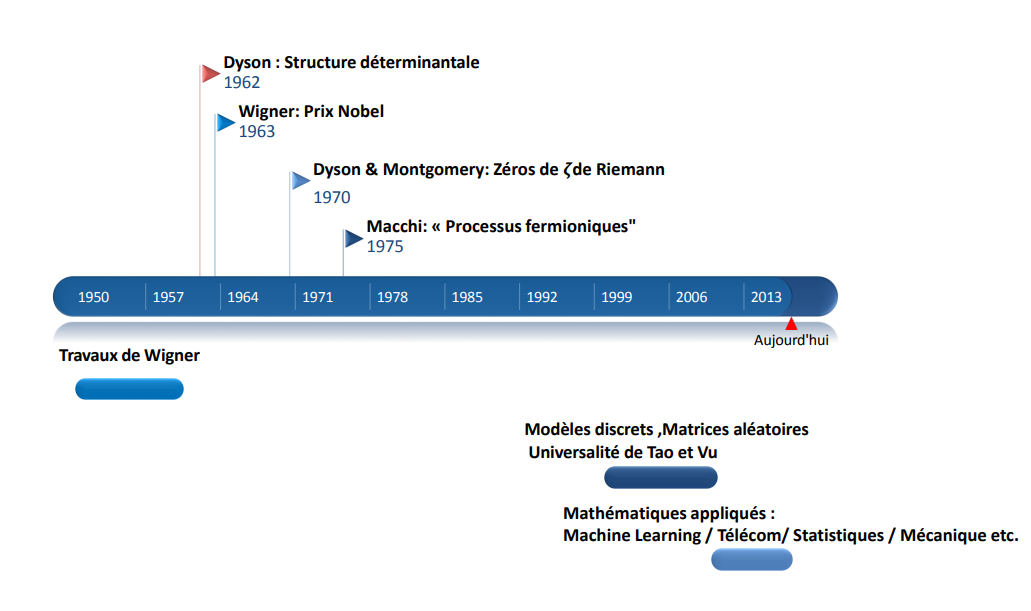
\includegraphics[scale=0.4]{Capture}
\end{frame}
\begin{frame}{Plan}
     \tableofcontents[
    hideothersubsections, 
    sectionstyle=show,
]
\end{frame}



\section{Objects combinatoires}
\begin{frame}{Plan}
\tableofcontents[currentsection,currentsubsection,
    hideothersubsections, 
    sectionstyle=show/shaded,
]
\end{frame}

\subsection{Plus longue sous-suite croissante}
\begin{frame}{Plus longue sous-suite croissante}
\begin{itemize}
    \item 
\item $\mathfrak{S_n}$ : Le groupe symétrique d'ordre $n$ (l'ensemble des permutations de $\{1,2,\dots,n\}$).
\\ 
\item $i_1<i_2<\dots<i_k$ est une sous-suite croissante de longueur $k$ si $\sigma(i_1)<\sigma(i_2)\dots\sigma(i_k)$.
\end{itemize}

\end{frame}
\subsection{blal}



\section{Objects combinatoires}
\begin{frame}{Plan}
\tableofcontents[currentsection,currentsubsection,
    hideothersubsections, 
    sectionstyle=show/shaded,
]
\end{frame}

\subsection{Conjecture d'Ulam}
\begin{frame}{test}
    
\end{frame}

\subsection{Theorème de Baik Deift Johannson}
\begin{frame}{test}
    
\end{frame}
\section{Universalité}
\begin{frame}{Plan}
\tableofcontents[currentsection,currentsubsection,
    hideothersubsections, 
    sectionstyle=show/shaded,
]
\end{frame}
\end{document}